% CA3 beamer deck  --  Material Design 3 redesign
% Compile from repo root (twice):
%   xelatex -interaction=nonstopmode -output-directory=docs docs/CA3_PRESENTATION.tex
\documentclass[aspectratio=169]{beamer}

\usepackage{fontspec}
\usepackage{amsmath,amssymb}
\usepackage{graphicx}
\usepackage{booktabs}
\usepackage{tabularx}
\usepackage{tikz}
\usepackage{colortbl}
\usetikzlibrary{arrows.meta,positioning}
\graphicspath{{outputs/figures/}{docs/figures/}{docs/assets/}}

% ---------- physics notation ----------
\newcommand{\pt}{p_{\mathrm{T}}}
\newcommand{\met}{E_{\mathrm{T}}^{\mathrm{miss}}}
\newcommand{\HT}{H_{T}}
\newcommand{\STlep}{S_{T}^{\ell}}
\newcommand{\njet}{N_{\mathrm{jets}}}

% ---------- Material Design 3 baseline palette ----------
\definecolor{MD3Primary}{RGB}{103,80,164}
\definecolor{MD3OnPrimary}{RGB}{255,255,255}
\definecolor{MD3PrimaryContainer}{RGB}{234,221,255}
\definecolor{MD3OnPrimaryContainer}{RGB}{33,0,93}
\definecolor{MD3Secondary}{RGB}{98,91,113}
\definecolor{MD3OnSecondary}{RGB}{255,255,255}
\definecolor{MD3SecondaryContainer}{RGB}{232,222,248}
\definecolor{MD3OnSecondaryContainer}{RGB}{29,25,43}
\definecolor{MD3Tertiary}{RGB}{125,82,96}
\definecolor{MD3OnTertiary}{RGB}{255,255,255}
\definecolor{MD3TertiaryContainer}{RGB}{255,216,228}
\definecolor{MD3OnTertiaryContainer}{RGB}{49,17,29}
\definecolor{MD3Error}{RGB}{179,38,30}
\definecolor{MD3OnError}{RGB}{255,255,255}
\definecolor{MD3ErrorContainer}{RGB}{249,222,220}
\definecolor{MD3OnErrorContainer}{RGB}{65,14,11}
\definecolor{MD3Surface}{RGB}{254,247,255}
\definecolor{MD3OnSurface}{RGB}{29,27,32}
\definecolor{MD3SurfaceVariant}{RGB}{231,224,236}
\definecolor{MD3OnSurfaceVariant}{RGB}{73,69,79}
\definecolor{MD3SurfaceContainerLow}{RGB}{243,237,247}
\definecolor{MD3SurfaceContainer}{RGB}{236,230,240}
\definecolor{MD3SurfaceContainerHigh}{RGB}{230,224,233}
\definecolor{MD3Outline}{RGB}{121,116,126}
\definecolor{MD3OutlineVariant}{RGB}{202,196,208}

% Dark colorful palette for tech badges
\definecolor{BadgeHadoop}{RGB}{19,102,118}
\definecolor{BadgeHive}{RGB}{140,85,15}
\definecolor{BadgeSpark}{RGB}{179,65,15}
\definecolor{BadgePig}{RGB}{138,43,88}
\definecolor{BadgeScikit}{RGB}{21,101,192}

% ---------- typography (MD3 type scale with Roboto) ----------
\setsansfont{Roboto}[
  Path = /usr/share/fonts/google-roboto/,
  Extension = .ttf,
  UprightFont = *-Regular,
  BoldFont = *-Medium,
  ItalicFont = *-Italic,
  BoldItalicFont = *-MediumItalic
]
\setmonofont{Liberation Mono}[Scale=MatchLowercase]

\setbeamerfont{normal text}{size=\fontsize{9.5}{13}\selectfont}
\setbeamerfont{frametitle}{size=\fontsize{15}{18}\selectfont,series=\bfseries}
\setbeamerfont{block title}{size=\fontsize{11}{14}\selectfont,series=\bfseries}
\setbeamerfont{block body}{size=\fontsize{9.5}{13}\selectfont}
\setbeamerfont{caption}{size=\fontsize{8}{10}\selectfont}
\setbeamerfont{footnote}{size=\fontsize{7.5}{9.5}\selectfont}

% ---------- MD3 color roles ----------
\setbeamercolor{normal text}{fg=MD3OnSurface,bg=MD3Surface}
\setbeamercolor{structure}{fg=MD3Primary}
\setbeamercolor{palette primary}{fg=MD3OnPrimary,bg=MD3Primary}
\setbeamercolor{palette secondary}{fg=MD3OnSecondary,bg=MD3Secondary}
\setbeamercolor{palette tertiary}{fg=MD3OnTertiary,bg=MD3Tertiary}
\setbeamercolor{palette quaternary}{fg=MD3OnSurfaceVariant,bg=MD3SurfaceContainerLow}
\setbeamercolor{frametitle}{fg=MD3OnSurface,bg=MD3Surface}
\setbeamercolor{block title}{fg=MD3OnSurface,bg=MD3SurfaceContainerHigh}
\setbeamercolor{block body}{fg=MD3OnSurfaceVariant,bg=MD3SurfaceContainerLow}
\setbeamercolor{block title example}{fg=MD3OnTertiaryContainer,bg=MD3TertiaryContainer}
\setbeamercolor{block body example}{fg=MD3OnSurfaceVariant,bg=MD3SurfaceContainerLow}
\setbeamercolor{block title alerted}{fg=MD3OnErrorContainer,bg=MD3ErrorContainer}
\setbeamercolor{block body alerted}{fg=MD3OnSurfaceVariant,bg=MD3SurfaceContainerLow}
\setbeamercolor{itemize item}{fg=MD3Primary}
\setbeamercolor{itemize subitem}{fg=MD3Secondary}
\setbeamercolor{itemize subsubitem}{fg=MD3Tertiary}
\setbeamercolor{enumerate item}{fg=MD3Primary}
\setbeamercolor{section in toc}{fg=MD3OnSurface}
\setbeamercolor{subsection in toc}{fg=MD3OnSurfaceVariant}
\setbeamercolor{caption}{fg=MD3OnSurfaceVariant}
\setbeamertemplate{navigation symbols}{}
\setbeamertemplate{blocks}[rounded][shadow=false]
\setbeamertemplate{caption}[numbered]
\setbeamertemplate{itemize item}{\scriptsize\textbullet}
\setbeamertemplate{itemize subitem}{\tiny$\circ$}
\setbeamertemplate{itemize subsubitem}{\tiny$\blacksquare$}
\setbeamertemplate{enumerate items}[default]
\hypersetup{colorlinks=true,linkcolor=MD3Primary,urlcolor=MD3Primary}
\arrayrulecolor{MD3OutlineVariant}
\renewcommand{\arraystretch}{1.25}

% ---------- MD3 top app bar (Small Top App Bar style) ----------
\setbeamertemplate{headline}{}
\setbeamertemplate{frametitle}{%
  \nointerlineskip%
  \vspace*{0.2cm}%
  \begin{beamercolorbox}[wd=\paperwidth,ht=4.2ex,dp=2.2ex,leftskip=0.6cm,rightskip=0.6cm]{frametitle}%
    {\usebeamerfont{frametitle}\color{MD3Primary}\raisebox{-0.15ex}{\insertframetitle}}%
    \hfill%
    \ifx\insertsection\empty\else%
      \tikz[baseline=-2pt]\node[rounded corners=7pt,fill=MD3PrimaryContainer,inner sep=4pt]{\color{MD3OnPrimaryContainer}\scriptsize\bfseries\insertsection};%
    \fi%
  \end{beamercolorbox}%
}

% ---------- MD3 bottom bar ----------
\setbeamertemplate{footline}{%
  \leavevmode%
  \begin{beamercolorbox}[wd=\paperwidth,ht=3ex,dp=1.5ex,leftskip=0.6cm,rightskip=0.6cm]{palette quaternary}%
    {\color{MD3OnSurfaceVariant}\scriptsize CA3 -- Big Data Analytics -- LHC 40\,MHz}%
    \hfill%
    \tikz[baseline=-2pt]\node[rounded corners=6pt,fill=MD3Primary,inner sep=3pt]{\color{MD3OnPrimary}\scriptsize\bfseries\insertframenumber};%
  \end{beamercolorbox}%
}

% ---------- MD3 components ----------
% filled tonal chip (8pt border radius, comfortable padding)
\newcommand{\mdchip}[3]{%
  \tikz[baseline=-2pt]\node[rounded corners=9pt,fill=#1,inner sep=5pt,minimum height=0.55cm]{\color{#2}\scriptsize\bfseries #3};}
% key-number card (rounded 12pt, surface container tone)
\newcommand{\mdnum}[4]{%
  \tikz[baseline=-2pt]\node[rounded corners=12pt,fill=#1,draw=MD3OutlineVariant,line width=0.5pt,inner sep=6pt,align=center,text width=#2,font=\scriptsize]{\color{#3}\bfseries #4};}
% figure inside MD3 rounded card (12pt corner, outline variant)
\newcommand{\mdfig}[2]{%
  \begin{tikzpicture}
    \node[rounded corners=10pt,fill=MD3SurfaceContainerLow,draw=MD3OutlineVariant,line width=0.5pt,inner sep=4pt] {%
      \includegraphics[#1]{#2}};
  \end{tikzpicture}}

\title{Big Data Analytics for LHC Event Quality and Exploratory Outlier Ranking in 40\,MHz Training Data}
\subtitle{CA-3 Case Study Presentation}
\author{Soham Kulkarni}
\institute[AIML B2]{Final Year AIML B2, 2023--27 \quad PRN 23070126129}
\date{Platforms: Hadoop $\cdot$ Hive $\cdot$ Spark 3.5.7 $\cdot$ Pig 0.17 $\cdot$ scikit-learn 1.6.1}

\begin{document}

% ============================================================ S1
\begin{frame}[plain]
  \begin{tikzpicture}[remember picture,overlay]
    \fill[MD3PrimaryContainer!70] (current page.north east) ++(-3.6,-1.6) circle (2.4cm);
    \fill[MD3TertiaryContainer!60] (current page.north east) ++(-1.6,-0.7) circle (1.1cm);
    \fill[MD3SecondaryContainer!50] (current page.south west) ++(2.8,1.6) circle (1.5cm);
    % Subtle LHC accelerator watermark
    \node[opacity=0.10] at ([xshift=-3.8cm,yshift=-2.2cm]current page.north east) {%
      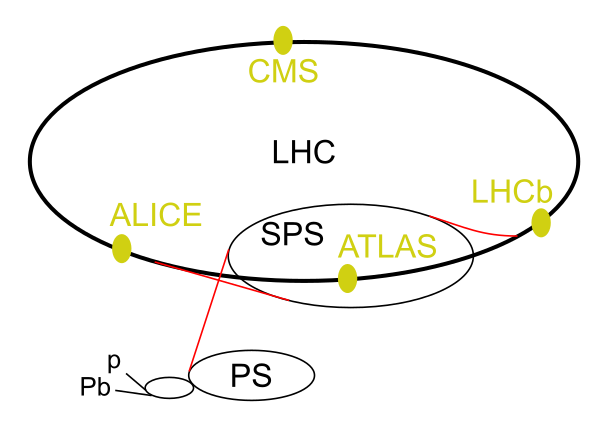
\includegraphics[width=6.2cm,keepaspectratio]{lhc.png}};
    % CERN crest top right
    \node[opacity=0.85] at ([xshift=-1.5cm,yshift=-1.1cm]current page.north east) {%
      
\includegraphics[height=0.95cm,keepaspectratio]{cern.png}};
  \end{tikzpicture}
  \vspace{0.6cm}
  \mdchip{MD3PrimaryContainer}{MD3OnPrimaryContainer}{CA-3 CASE STUDY}
  \\[0.35cm]
  {\fontsize{20}{24}\selectfont\bfseries\color{MD3OnSurface} Big Data Analytics for LHC Event Quality\\[0.25em] and Exploratory Outlier Ranking in 40\,MHz Training Data}
  \\[0.35cm]
  {\fontsize{11}{14}\selectfont\color{MD3OnSurfaceVariant} Big Data Analytics CA-3 Case Study Presentation}
  \\[0.5cm]
  {\fontsize{9.5}{12}\selectfont\color{MD3OnSurface} Soham Kulkarni $\cdot$ PRN 23070126129 $\cdot$ AIML B2, 2023--27}
  \\[0.4cm]
  \mdchip{BadgeHadoop}{white}{Hadoop}\hspace{0.25cm}%
  \mdchip{BadgeHive}{white}{Hive}\hspace{0.25cm}%
  \mdchip{BadgeSpark}{white}{Spark 3.5.7}\hspace{0.25cm}%
  \mdchip{BadgePig}{white}{Pig 0.17}\hspace{0.25cm}%
  \mdchip{BadgeScikit}{white}{scikit-learn 1.6.1}
\end{frame}

% ============================================================ S2
\section{Introduction}
\begin{frame}{Agenda}
  \vspace{0.15cm}
  \begin{columns}[T]
    \begin{column}{0.48\textwidth}
      \begin{block}{Phase 1 -- Foundation \& Ingestion}
        \footnotesize
        \begin{enumerate}
          \item \textbf{Introduction} (Problem \& Deliverables)
          \item \textbf{Dataset \& Schema} (Zenodo \& 13.45M Rows)
          \item \textbf{Pipeline} (Architecture \& Scaling)
          \item \textbf{Quality \& Distributions} (Zero-Defect Audit)
        \end{enumerate}
      \end{block}
    \end{column}
    \begin{column}{0.48\textwidth}
      \begin{block}{Phase 2 -- Computation \& Insights}
        \footnotesize
        \begin{enumerate}
          \setcounter{enumi}{4}
          \item \textbf{Spark Analytics} (9 SQL Queries \& RDD)
          \item \textbf{Ecosystem} (Hadoop, Hive \& Pig Integration)
          \item \textbf{Unsupervised Scoring} (MiniBatchKMeans)
          \item \textbf{Synthesis} (Engineering Results \& Summary)
        \end{enumerate}
      \end{block}
    \end{column}
  \end{columns}
\end{frame}

% ============================================================ S3
\begin{frame}{Problem Statement}
  \begin{columns}[T]
    \begin{column}{0.54\textwidth}
      \begin{block}{\raisebox{-0.05cm}{
\includegraphics[height=0.34cm]{atom.png}}\hspace{0.12cm}Trigger-level Setting}
        \footnotesize
        \begin{itemize}
          \item LHC bunch crossings @ \textbf{40\,MHz} (25\,ns interval)
          \item Online L1 trigger discards bulk before storage
          \item Reconstructed physics objects: e$^\pm$, $\mu^\pm$, jets, $\met$
        \end{itemize}
      \end{block}
      \begin{block}{\raisebox{-0.05cm}{
\includegraphics[height=0.34cm]{microchip.png}}\hspace{0.12cm}Research Question}
        \footnotesize
        Can an auditable bounded-memory pipeline validate full HDF5 tensors, build typed Parquet tables, and rank atypical events on 6 CPU cores?
      \end{block}
    \end{column}
    \begin{column}{0.42\textwidth}
      \begin{exampleblock}{\raisebox{-0.05cm}{
\includegraphics[height=0.34cm]{diagram-project.png}}\hspace{0.12cm}Pipeline Deliverables}
        \footnotesize
        \begin{itemize}
          \item Quality gate: full-corpus zero-defect audit
          \item Spark SQL + RDD analytics on single-node Docker
          \item Unsupervised mini-batch distance scoring
        \end{itemize}
      \end{exampleblock}
      \vspace{0.2cm}
      \mdnum{MD3Primary}{4.4cm}{MD3OnPrimary}{646.4\,MB HDF5 source \\ 13.45M events verified}
    \end{column}
  \end{columns}
\end{frame}

% ============================================================ S4
\section{Dataset \& Schema}
\begin{frame}{Dataset \& Provenance}
  \begin{columns}[T]
    \begin{column}{0.54\textwidth}
      \tiny
      \begin{tabularx}{\textwidth}{l X}
        \toprule
        \rowcolor{MD3SurfaceContainer}
        \textbf{Property} & \textbf{Value} \\
        \midrule
        Repository & Zenodo 5046428 (DOI 10.5281/zenodo.5046428) \\
        File & \texttt{background\_for\_training.h5} (646.39\,MB) \\
        MD5 & \texttt{08cb4801229f9d480567f8d3f5cac134} \checkmark \\
        SHA-256 & \texttt{5f460bd3af44\ldots cfe5} \\
        Keys & \texttt{/Particles}, \texttt{\_Names}, \texttt{\_Classes} \\
        Storage & float64, gzip-4, chunks (26274,1,1) \\
        \bottomrule
      \end{tabularx}
      \vspace{0.15cm}
      \begin{exampleblock}{\raisebox{-0.05cm}{
\includegraphics[height=0.32cm]{database.png}}\hspace{0.12cm}Raw Scale}
        \scriptsize
        $13{,}451{,}915 \times 19 \times 4 = 1{,}022{,}345{,}540$ scalars \\
        $\times\,8$\,B $= 8.18$\,GB uncompressed ($\approx 12.7\times$ gzip ratio)
      \end{exampleblock}
    \end{column}
    \begin{column}{0.42\textwidth}
      \begin{exampleblock}{Audited Cardinality}
        \footnotesize
        \begin{itemize}
          \item Dataset paper states \textbf{4,000,000} events
          \item File scan yields \textbf{13,451,915} rows
          \item Pipeline evaluates 100\% without subsampling
        \end{itemize}
      \end{exampleblock}
      \vspace{0.15cm}
      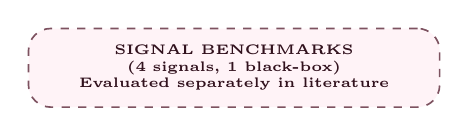
\begin{tikzpicture}
        \node[rounded corners=8pt,draw=MD3Tertiary,line width=0.6pt,dashed,fill=MD3TertiaryContainer!30,align=center,inner sep=6pt,text width=4.8cm,font=\tiny\bfseries,text=MD3OnTertiaryContainer] {SIGNAL BENCHMARKS (4 signals, 1 black-box)\\Evaluated separately in literature};
      \end{tikzpicture}
    \end{column}
  \end{columns}
\end{frame}

% ============================================================ S5
\begin{frame}{Fixed-Width Tensor Schema}
  \begin{columns}[T]
    \begin{column}{0.50\textwidth}
      \begin{figure}
        \centering
        \mdfig{height=0.38\textheight,keepaspectratio}{documented_tensor_schema.png}
        \caption{Documented $19\times4$ slot layout ([$\pt$, $\eta$, $\phi$, type]).}
      \end{figure}
    \end{column}
    \begin{column}{0.46\textwidth}
      \tiny
      \begin{tabularx}{\textwidth}{c l c}
        \toprule
        \rowcolor{MD3SurfaceContainer}
        \textbf{Slots} & \textbf{Segment} & \textbf{Code} \\
        \midrule
        0 & MET ($E_{\mathrm{T}}^{\mathrm{miss}}$) & $t{=}1$ \\
        1--4 & electrons (max 4) & $t{=}2$ \\
        5--8 & muons (max 4) & $t{=}3$ \\
        9--18 & jets (max 10) & $t{=}4$ \\
        unused & zero-padding & $t{=}0$ \\
        \bottomrule
      \end{tabularx}
      \vspace{0.15cm}
      \begin{block}{Validation Rules}
        \scriptsize
        \begin{itemize}
          \item Objects sorted by descending $\pt$ within group
          \item Padding rule: $t_i=0 \Rightarrow \pt{=}\eta{=}\phi{=}0.0$
          \item Type code gate: finite $\wedge$ integer $\in\{0,\dots,4\}$
          \item Schema assertion: \texttt{ndim==3}, shape[1:] $=(19,4)$
        \end{itemize}
      \end{block}
    \end{column}
  \end{columns}
\end{frame}

% ============================================================ S6
\begin{frame}{Physics Context}
  \begin{columns}[T]
    \begin{column}{0.48\textwidth}
      \begin{block}{Standard Model process mixture (published)}
        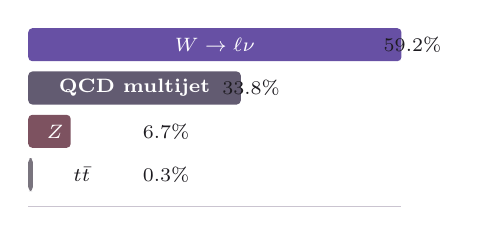
\begin{tikzpicture}
          \fill[MD3Primary,rounded corners=1.5pt] (0,0) rectangle (4.74,0.42);
          \node[font=\scriptsize\bfseries,text=MD3OnPrimary] at (2.37,0.21) {$W\to\ell\nu$};
          \node[font=\scriptsize,text=MD3OnSurface] at (4.88,0.21) {59.2\%};
          \fill[MD3Secondary,rounded corners=1.5pt] (0,-0.55) rectangle (2.70,-0.13);
          \node[font=\scriptsize\bfseries,text=MD3OnSecondary] at (1.35,-0.34) {QCD multijet};
          \node[font=\scriptsize,text=MD3OnSurface] at (2.83,-0.34) {33.8\%};
          \fill[MD3Tertiary,rounded corners=1.5pt] (0,-1.10) rectangle (0.54,-0.68);
          \node[font=\scriptsize\bfseries,text=MD3OnTertiary] at (0.68,-0.89) {$Z\to\ell\ell$};
          \node[font=\scriptsize,text=MD3OnSurface] at (1.75,-0.89) {6.7\%};
          \fill[MD3Outline,rounded corners=1.5pt] (0,-1.65) rectangle (0.06,-1.23);
          \node[font=\scriptsize\bfseries,text=MD3OnSurface] at (0.68,-1.44) {$t\bar{t}$};
          \node[font=\scriptsize,text=MD3OnSurface] at (1.75,-1.44) {0.3\%};
          \draw[MD3OutlineVariant] (0,-1.85) -- (4.74,-1.85);
        \end{tikzpicture}
      \end{block}
      \begin{block}{Simulation \& Selection}
        \tiny 13\,TeV $pp$, PYTHIA + DELPHES sim; single-lepton trigger selection.
      \end{block}
    \end{column}
    \begin{column}{0.48\textwidth}
      \begin{block}{Kinematics Conventions}
        \tiny
        \begin{align*}
          \pt &= \sqrt{p_x^2+p_y^2} \quad [\text{GeV}], \quad \eta = -\ln[\tan(\theta/2)]\\
          \HT &= \textstyle\sum_{\text{jets}} p_{\mathrm{T},i}, \quad \STlep = \textstyle\sum_{e,\mu} p_{\mathrm{T},i}
        \end{align*}
        $\met$\ magnitude read directly from fixed slot 0.
      \end{block}
      \vspace{0.05cm}
      \begin{exampleblock}{Species Mapping}
        \tiny
        
\begin{tikzpicture}[every node/.style={font=\tiny\bfseries}]
          \node[rounded corners=4pt,fill=BadgeHadoop,text=white,inner sep=2.5pt] (met) at (0,0) {$\met$\,(1)};
          \node[rounded corners=4pt,fill=BadgeScikit,text=white,inner sep=2.5pt] (e) at (1.2,0) {$e^\pm$\,(2)};
          \node[rounded corners=4pt,fill=BadgePig,text=white,inner sep=2.5pt] (mu) at (2.2,0) {$\mu^\pm$\,(3)};
          \node[rounded corners=4pt,fill=BadgeSpark,text=white,inner sep=2.5pt] (jet) at (3.3,0) {jet\,(4)};
          \node[rounded corners=4pt,fill=MD3Outline,text=white,inner sep=2.5pt] (pad) at (4.4,0) {pad\,(0)};
        \end{tikzpicture}
      \end{exampleblock}
    \end{column}
  \end{columns}
\end{frame}

% ============================================================ S7
\section{Pipeline}
\begin{frame}{System Architecture}
  \centering
  \begin{tikzpicture}[
      >=Stealth, every node/.style={font=\scriptsize},
      stageN/.style={rectangle,rounded corners=5pt,draw=MD3Outline,fill=MD3SurfaceContainerLow,line width=0.7pt,text width=2.3cm,minimum height=1.15cm,align=center,inner sep=3pt},
      engineN/.style={rectangle,rounded corners=5pt,draw=MD3Primary,fill=MD3PrimaryContainer,line width=0.7pt,text width=2.8cm,minimum height=1.1cm,align=center,inner sep=3pt,text=MD3OnPrimaryContainer},
      wideN/.style={rectangle,rounded corners=5pt,draw=MD3Secondary,fill=MD3SecondaryContainer,line width=0.7pt,text width=12.4cm,minimum height=0.75cm,align=center,inner sep=3pt,text=MD3OnSecondaryContainer},
      dashN/.style={rectangle,rounded corners=5pt,draw=MD3Outline,fill=MD3Surface,line width=0.7pt,dashed,text width=12.4cm,minimum height=0.75cm,align=center,inner sep=3pt,text=MD3OnSurfaceVariant},
      arr/.style={->,draw=MD3Primary,line width=0.9pt},
      engArr/.style={->,draw=MD3Secondary,line width=0.9pt},
      optArr/.style={->,dashed,draw=MD3Outline,line width=0.7pt}
    ]
    \node[stageN] (S1) at (0,0) {\textbf{1. Zenodo ingest}\\646.4\,MB HDF5\\MD5+size gate};
    \node[stageN] (S2) at (3.5,0) {\textbf{2. Quality gate}\\1.02B scalars\\539 chunks};
    \node[stageN] (S3) at (7.0,0) {\textbf{3. Feature ETL}\\13.45M rows\\17 columns};
    \node[stageN] (S4) at (10.5,0) {\textbf{4. Parquet store}\\624.78\,MB Snappy\\539 row groups};
    \draw[arr] (S1) -- (S2);
    \draw[arr] (S2) -- (S3);
    \draw[arr] (S3) -- (S4);
    \node[engineN] (E1) at (1.4,-1.75) {\textbf{Spark SQL}\hspace{0.15cm}\raisebox{-0.15cm}{
\includegraphics[height=0.48cm,keepaspectratio]{spark.png}}\\9 HiveQL-compatible\\queries};
    \node[engineN] (E2) at (5.6,-1.75) {\textbf{Spark RDD}\hspace{0.15cm}\raisebox{-0.15cm}{
\includegraphics[height=0.48cm,keepaspectratio]{spark.png}}\\map $\to$ reduceByKey\\key $= \njet$};
    \node[engineN] (E3) at (9.8,-1.75) {\textbf{MiniBatchKMeans}\hspace{0.15cm}\raisebox{-0.15cm}{
\includegraphics[height=0.45cm,keepaspectratio]{scikit.png}}\\$K{=}8$, 10 features\\anomaly scoring};
    \draw[arr] (S4.south) -- ++(0,-0.30);
    \draw[arr,-] (10.5,-0.62) -- (1.4,-0.62);
    \draw[arr] (1.4,-0.62) -- (E1.north);
    \draw[arr] (5.6,-0.62) -- (E2.north);
    \draw[arr] (9.8,-0.62) -- (E3.north);
    \node[wideN] (OUT) at (5.6,-3.15) {\textbf{Evidence \& output manifests}\\9 figures (PNG+SVG) $\bullet$ 9 CSV result dirs $\bullet$ JSON run manifests $\bullet$ \texttt{cluster\_scores.parquet}};
    \draw[engArr] (E1.south) -- (E1.south |- OUT.north);
    \draw[engArr] (E2.south) -- (OUT.north);
    \draw[engArr] (E3.south) -- (E3.south |- OUT.north);
    \node[dashN] (OPT) at (5.6,-4.35) {\textbf{Optional ecosystem}: \raisebox{-0.10cm}{
\includegraphics[height=0.45cm]{hadoop.png}}\hspace{0.15cm}Hadoop Streaming $\bullet$ \raisebox{-0.10cm}{
\includegraphics[height=0.45cm]{hive.png}}\hspace{0.15cm}Hive DDL $\bullet$ \raisebox{-0.10cm}{
\includegraphics[height=0.45cm]{pig.png}}\hspace{0.15cm}Pig 0.17};
    \draw[optArr] (OUT.south) -- (OPT.north);
  \end{tikzpicture}
  \\
  \scriptsize Row 1 = core path $\cdot$ Row 2 = parallel engines via distribution bus $\cdot$ Row 4 = external-infra artefacts
\end{frame}


% ============================================================ S8
\begin{frame}{Methodology -- Pipeline Architecture}
  \begin{columns}[T]
    \begin{column}{0.50\textwidth}
      \begin{block}{Quality-first Design}
        \footnotesize
        \begin{enumerate}
          \item Full checksum \& provenance check
          \item Schema assertion prior to ETL
          \item 1:1 row correspondence throughout
        \end{enumerate}
      \end{block}
      \begin{block}{Bounded-memory Execution}
        \footnotesize
        Fixed streaming chunks of 25{,}000 rows (539 row groups); peak container RSS $\le 8$\,GB.
      \end{block}
    \end{column}
    \begin{column}{0.46\textwidth}
      \begin{exampleblock}{Parity Validation}
        \footnotesize
        \begin{itemize}
          \item ETL: 13{,}451{,}915 in $=$ 13{,}451{,}915 out
          \item Spark: partition sum $=$ 13{,}451{,}915
          \item RDD: $\sum n_j = 13{,}451{,}915$
          \item ML: 100\% rows scored without loss
        \end{itemize}
      \end{exampleblock}
      \vspace{0.1cm}
      \scriptsize Timings: Spark 93.8\,s $\cdot$ ML 25.2\,s (single host, 6 cores).
    \end{column}
  \end{columns}
\end{frame}

% ============================================================ S9
\section{Quality \& Distributions}
\begin{frame}{Data Quality Gate (Full-Corpus Audit)}
  \begin{columns}[T]
    \begin{column}{0.52\textwidth}
      \begin{block}{Defect Counters (1.02B Scalars Scanned)}
        \tiny
        \begin{tabularx}{\textwidth}{X r}
          \toprule
          \rowcolor{MD3SurfaceContainer}
          \textbf{Integrity Check} & \textbf{Count} \\
          \midrule
          NaN entries & 0 \\
          $+\infty$ / $-\infty$ entries & 0 / 0 \\
          Invalid type code $\notin\{0..4\}$ & 0 \\
          Non-integral type code & 0 \\
          Negative occupied $\pt$ & 0 \\
          $|\phi|>\pi$ out-of-range & 0 \\
          Nonzero padding kinematics & 0 \\
          Misplaced slot code & 0 \\
          \midrule
          \textbf{Total defects} & \textbf{0} \\
          \bottomrule
        \end{tabularx}
      \end{block}
    \end{column}
    \begin{column}{0.44\textwidth}
      \begin{block}{Slot Occupancy (255.6M slots)}
        \centering
        
\begin{tikzpicture}
          \fill[MD3Primary,rounded corners=1.5pt] (0,0) rectangle (0.9,0.4);
          \fill[MD3OutlineVariant,rounded corners=1.5pt] (0.9,0) rectangle (5.0,0.4);
          \node[font=\tiny,MD3OnPrimaryContainer,align=center] at (0.45,0.55) {occupied};
          \node[font=\tiny,MD3OnSurfaceVariant,align=center] at (3.0,0.55) {structural zero padding};
          \node[font=\tiny,MD3OnPrimary] at (3.0,0.2) {82.83\%};
        \end{tikzpicture}
        \vspace{0.05cm}
        \\
        \tiny 100\% of events contain valid zero-padding.
      \end{block}
      \vspace{0.1cm}
      \mdnum{MD3Tertiary}{4.6cm}{MD3OnTertiary}{\raisebox{-0.06cm}{
\includegraphics[height=0.36cm]{shield.png}}\hspace{0.15cm}0 defects \\ 100\% clean data gate}
    \end{column}
  \end{columns}
\end{frame}

% ============================================================ S10
\begin{frame}{Object Multiplicity (All 13.45M Events)}
  \centering
  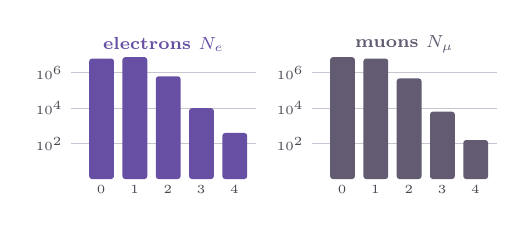
\begin{tikzpicture}[scale=0.9,every node/.style={transform shape}]
    % ---- electrons ----
    \draw[MD3OutlineVariant] (0,0.5) -- (2.6,0.5); \draw[MD3OutlineVariant] (0,1.0) -- (2.6,1.0); \draw[MD3OutlineVariant] (0,1.5) -- (2.6,1.5);
    \node[font=\tiny,MD3OnSurfaceVariant,anchor=east] at (0,0.5) {$10^2$};
    \node[font=\tiny,MD3OnSurfaceVariant,anchor=east] at (0,1.0) {$10^4$};
    \node[font=\tiny,MD3OnSurfaceVariant,anchor=east] at (0,1.5) {$10^6$};
    \foreach \x/\h/\l in {0.25/1.7/0,0.72/1.72/1,1.19/1.45/2,1.66/1.0/3,2.13/0.65/4}{
      \fill[MD3Primary,rounded corners=1pt] (\x,0) rectangle (\x+0.35,\h);
      \node[font=\tiny,MD3OnSurfaceVariant] at (\x+0.17,-0.15) {\l};}
    \node[font=\scriptsize\bfseries,MD3Primary] at (1.3,1.9) {electrons $N_e$};
    % ---- muons ----
    \begin{scope}[xshift=3.4cm]
      \draw[MD3OutlineVariant] (0,0.5) -- (2.6,0.5); \draw[MD3OutlineVariant] (0,1.0) -- (2.6,1.0); \draw[MD3OutlineVariant] (0,1.5) -- (2.6,1.5);
      \node[font=\tiny,MD3OnSurfaceVariant,anchor=east] at (0,0.5) {$10^2$};
      \node[font=\tiny,MD3OnSurfaceVariant,anchor=east] at (0,1.0) {$10^4$};
      \node[font=\tiny,MD3OnSurfaceVariant,anchor=east] at (0,1.5) {$10^6$};
      \foreach \x/\h/\l in {0.25/1.72/0,0.72/1.7/1,1.19/1.42/2,1.66/0.95/3,2.13/0.55/4}{
        \fill[MD3Secondary,rounded corners=1pt] (\x,0) rectangle (\x+0.35,\h);
        \node[font=\tiny,MD3OnSurfaceVariant] at (\x+0.17,-0.15) {\l};}
      \node[font=\scriptsize\bfseries,MD3Secondary] at (1.3,1.9) {muons $N_\mu$};
    \end{scope}
  \end{tikzpicture}
  \\[0.1cm]
  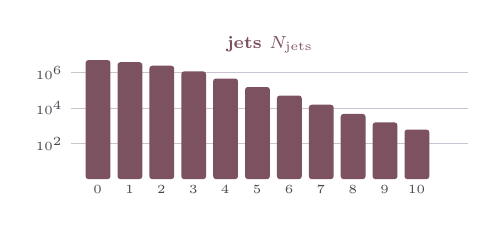
\begin{tikzpicture}[scale=0.9,every node/.style={transform shape}]
    % ---- jets ----
    \draw[MD3OutlineVariant] (0,0.5) -- (5.6,0.5); \draw[MD3OutlineVariant] (0,1.0) -- (5.6,1.0); \draw[MD3OutlineVariant] (0,1.5) -- (5.6,1.5);
    \node[font=\tiny,MD3OnSurfaceVariant,anchor=east] at (0,0.5) {$10^2$};
    \node[font=\tiny,MD3OnSurfaceVariant,anchor=east] at (0,1.0) {$10^4$};
    \node[font=\tiny,MD3OnSurfaceVariant,anchor=east] at (0,1.5) {$10^6$};
    \foreach \x/\h/\l in {0.2/1.68/0,0.65/1.65/1,1.1/1.6/2,1.55/1.52/3,2.0/1.42/4,2.45/1.3/5,2.9/1.18/6,3.35/1.05/7,3.8/0.92/8,4.25/0.8/9,4.7/0.7/10}{
      \fill[MD3Tertiary,rounded corners=1pt] (\x,0) rectangle (\x+0.35,\h);
      \node[font=\tiny,MD3OnSurfaceVariant] at (\x+0.17,-0.15) {\l};}
    \node[font=\scriptsize\bfseries,MD3Tertiary] at (2.8,1.9) {jets $\njet$};
  \end{tikzpicture}
  \\[0.05cm]
  \scriptsize Log-scale multiplicity. $\njet\le 2$ covers \textbf{86.0\%} of events; tail reaches $\njet{=}10$ (731 events).
\end{frame}

% ============================================================ S11
\begin{frame}{Transverse-Momentum Spectra by Object Class}
  \begin{figure}
    \centering
    \mdfig{height=0.48\textheight,keepaspectratio}{01_pt_spectrum_by_object_type.png}
    \caption{Log-scale $\pt$ histograms per particle class (all 43.88M occupied slots). Trigger threshold $\pt>23$\,GeV visible; spectra peak at 20--50\,GeV.}
  \end{figure}
\end{frame}

% ============================================================ S12
\begin{frame}{MET vs Jet Activity (Joint Density)}
  \begin{columns}[T]
    \begin{column}{0.58\textwidth}
      \begin{figure}
        \centering
        \mdfig{height=0.45\textheight,keepaspectratio}{03_met_vs_jet_ht_density.png}
        \caption{Log-scale 2D hexbin density across all 13.45M events.}
      \end{figure}
    \end{column}
    \begin{column}{0.38\textwidth}
      \begin{block}{Phase Space Characteristics}
        \footnotesize
        \begin{itemize}
          \item Core bulk: $\met<50$\,GeV $\wedge$ $\HT<100$\,GeV
          \item Conditional median $\HT$ increases with $\met$
          \item Sparse high-activity tail flagged for review
        \end{itemize}
      \end{block}
      \vspace{0.15cm}
      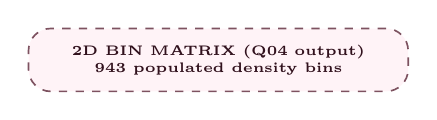
\begin{tikzpicture}
        \node[rounded corners=8pt,draw=MD3Tertiary,line width=0.6pt,dashed,fill=MD3TertiaryContainer!30,align=center,inner sep=6pt,text width=4.4cm,font=\tiny\bfseries,text=MD3OnTertiaryContainer] {2D BIN MATRIX (Q04 output)\\943 populated density bins};
      \end{tikzpicture}
    \end{column}
  \end{columns}
\end{frame}

% ============================================================ S13
\begin{frame}{Scalar Jet Activity Conditioned on $\njet$}
  \begin{columns}[T]
    \begin{column}{0.58\textwidth}
      \begin{figure}
        \centering
        \mdfig{height=0.45\textheight,keepaspectratio}{04_ht_by_jet_multiplicity.png}
        \caption{$\HT$ distribution conditioned on jet multiplicity ($0$--$10$).}
      \end{figure}
    \end{column}
    \begin{column}{0.38\textwidth}
      \begin{block}{Multiplicity Trends}
        \footnotesize
        \begin{itemize}
          \item Median $\HT$ scales from 0 to 652.9\,GeV
          \item Spread expands at higher jet counts
          \item Exactly zero $\HT$ for 5.08M zero-jet events
        \end{itemize}
      \end{block}
      \vspace{0.15cm}
      \mdnum{MD3Secondary}{4.4cm}{MD3OnSecondary}{652.9\,GeV median $\HT$ \\ at $\njet{=}10$}
    \end{column}
  \end{columns}
\end{frame}

% ============================================================ S14
\begin{frame}{Feature Correlations}
  \begin{columns}[T]
    \begin{column}{0.48\textwidth}
      \begin{figure}
        \centering
        \mdfig{width=0.92\linewidth,height=0.36\textheight,keepaspectratio}{06_feature_correlations.png}
        \caption{Feature correlations (13.45M rows).}
      \end{figure}
    \end{column}
    \begin{column}{0.46\textwidth}
      \begin{exampleblock}{Key Coefficients}
        \footnotesize
        \begin{itemize}
          \item $\HT$--$\njet$: $r{=}0.74$, $\rho{=}0.87$
          \item $\met$--$\HT$: $r{=}0.15$ (orthogonal)
        \end{itemize}
      \end{exampleblock}
      \vspace{0.1cm}
      \begin{block}{Interpretation}
        \tiny $\HT$--$\njet$ correlation is construction-driven ($\HT = \sum \pt$). Weak $\met$--$\HT$ correlation confirms independent observables.
      \end{block}
    \end{column}
  \end{columns}
\end{frame}

% ============================================================ S15
\begin{frame}{Full-Corpus $\HT$ Distribution}
  \begin{columns}[T]
    \begin{column}{0.50\textwidth}
      \begin{figure}
        \centering
        \mdfig{height=0.40\textheight,keepaspectratio}{07_full_corpus_ht_distribution.png}
        \caption{$\HT$ distribution with signed-log axis.}
      \end{figure}
    \end{column}
    \begin{column}{0.44\textwidth}
      \begin{block}{Distribution Characteristics}
        \footnotesize
        \begin{itemize}
          \item Exact delta spike: 5.08M events at $\HT{=}0$
          \item Physical tail extends beyond 4{,}000\,GeV
          \item Log-scale display captures dynamic range
        \end{itemize}
      \end{block}
    \end{column}
  \end{columns}
\end{frame}

% ============================================================ S16
\section{Spark Analytics}
\begin{frame}{Spark SQL Query Suite}
  \tiny
  \begin{tabularx}{\textwidth}{c l X r}
    \toprule
    \rowcolor{MD3SurfaceContainer}
    \textbf{ID} & \textbf{Script} & \textbf{Key Operations} & \textbf{Rows} \\
    \midrule
    Q01 & \texttt{01\_dataset\_overview.sql} & COUNT, SUM, AVG, \texttt{percentile\_approx} & 1 \\
    Q02 & \texttt{02\_object\_multiplicity.sql} & Multiplicity distributions (e, $\mu$, jets) & 21 \\
    Q03 & \texttt{03\_ht\_by\_jet\_multiplicity.sql} & Conditional quartiles \& Pearson correlation & 11 \\
    Q04 & \texttt{04\_met\_ht\_density\_bins.sql} & 2D binning (20\,GeV $\times$ 50\,GeV cells) & 943 \\
    Q05 & \texttt{05\_quality\_flags.sql} & Quality gate flag verification & 1 \\
    Q06 & \texttt{06\_high\_activity\_candidates.sql} & Extreme activity event candidates ($\HT$ top 100) & 100 \\
    Q07 & \texttt{07\_feature\_correlation.sql} & Grouped feature correlations vs $\njet$ & 11 \\
    Q08 & \texttt{08\_window\_jet\_slice\_rankings.sql} & Window functions (\texttt{DENSE\_RANK}) top-3 per slice & 30 \\
    Q09 & \texttt{09\_multidimensional\_rollup.sql} & Multidimensional grouping (\texttt{ROLLUP}) & 28 \\
    \bottomrule
  \end{tabularx}
  \vspace{0.15cm}
  \begin{columns}[T]
    \begin{column}{0.48\textwidth}
      \begin{exampleblock}{\raisebox{-0.05cm}{
\includegraphics[height=0.32cm]{diagram-project.png}}\hspace{0.12cm}Runtime Execution Contract}
        \tiny Spark 3.5.7 \raisebox{-0.06cm}{
\includegraphics[height=0.35cm]{spark.png}}\hspace{0.1cm}\texttt{local[6]} $\cdot$ 12 partitions $\cdot$ AQE on $\cdot$ \textbf{93.8\,s} suite runtime.
      \end{exampleblock}
    \end{column}
    \begin{column}{0.48\textwidth}
      \begin{block}{\raisebox{-0.05cm}{
\includegraphics[height=0.32cm]{check.png}}\hspace{0.12cm}Parity Verification}
        \tiny All queries read typed Parquet with 1:1 row parity against raw audit.
      \end{block}
    \end{column}
  \end{columns}
\end{frame}

% ============================================================ S17
\begin{frame}{MapReduce Key-Value Aggregation (RDD)}
  \begin{columns}[T]
    \begin{column}{0.56\textwidth}
      \centering
      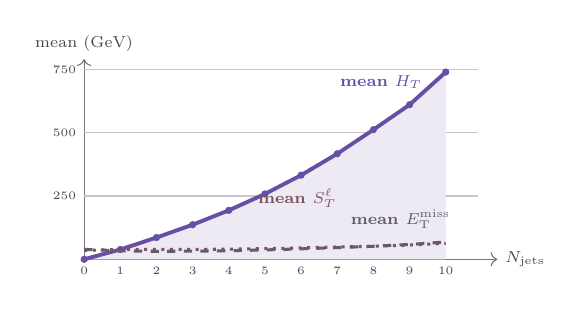
\begin{tikzpicture}[scale=0.82,every node/.style={transform shape}]
        % axes
        \draw[->,MD3Outline] (0,0) -- (6.4,0) node[right,font=\scriptsize,MD3OnSurfaceVariant]{$\njet$};
        \draw[->,MD3Outline] (0,0) -- (0,3.1) node[above,font=\scriptsize,MD3OnSurfaceVariant]{mean (GeV)};
        \foreach \y/\l in {0.98/250,1.96/500,2.94/750}{
          \draw[MD3OutlineVariant] (0,\y) -- (6.1,\y);
          \node[font=\tiny,MD3OnSurfaceVariant,anchor=east] at (0,\y) {\l};}
        % HT area + line
        \fill[MD3Primary!12] (0,0) -- (0.56,0.152) -- (1.12,0.337) -- (1.68,0.536) -- (2.24,0.758)
          -- (2.80,1.012) -- (3.36,1.303) -- (3.92,1.635) -- (4.48,2.008)
          -- (5.04,2.394) -- (5.60,2.900) -- (5.60,0) -- cycle;
        \draw[MD3Primary,line width=1.4pt]
          (0,0) -- (0.56,0.152) -- (1.12,0.337) -- (1.68,0.536) -- (2.24,0.758)
          -- (2.80,1.012) -- (3.36,1.303) -- (3.92,1.635) -- (4.48,2.008)
          -- (5.04,2.394) -- (5.60,2.900);
        \foreach \x/\y in {0/0,0.56/0.152,1.12/0.337,1.68/0.536,2.24/0.758,2.80/1.012,3.36/1.303,3.92/1.635,4.48/2.008,5.04/2.394,5.60/2.900}{
          \fill[MD3Primary] (\x,\y) circle (1.6pt);}
        % MET line
        \draw[MD3Secondary,line width=1.1pt,dashed]
          (0,0.154) -- (0.56,0.131) -- (1.12,0.124) -- (1.68,0.126) -- (2.24,0.133)
          -- (2.80,0.145) -- (3.36,0.162) -- (3.92,0.181) -- (4.48,0.202)
          -- (5.04,0.230) -- (5.60,0.268);
        % S_l line
        \draw[MD3Tertiary,line width=1.1pt,dotted]
          (0,0.136) -- (0.56,0.154) -- (1.12,0.152) -- (1.68,0.153) -- (2.24,0.157)
          -- (2.80,0.165) -- (3.36,0.176) -- (3.92,0.191) -- (4.48,0.202)
          -- (5.04,0.221) -- (5.60,0.248);
        \foreach \x in {0,...,10}{
          \node[font=\tiny,MD3OnSurfaceVariant] at ({\x*0.56},-0.18) {\x};}
        \node[font=\scriptsize,MD3Primary] at (4.6,2.75) {\textbf{mean $\HT$}};
        \node[font=\scriptsize,MD3Secondary] at (4.9,0.62) {\textbf{mean $\met$}};
        \node[font=\scriptsize,MD3Tertiary] at (3.3,0.95) {\textbf{mean $\STlep$}};
      \end{tikzpicture}
      \\
      \tiny RDD \texttt{map} $\to$ \texttt{reduceByKey} means (13.45M events).
    \end{column}
    \begin{column}{0.40\textwidth}
      \begin{block}{Algorithm Specification}
        \tiny
        \begin{align*}
          \text{Map}(e) &\mapsto \bigl(\njet,\ (1,\HT,\met,\STlep)\bigr)\\
          \text{Reduce} &: (n,s_H,s_M,s_L)\oplus(n',s'_H,s'_M,s'_L)\\
          &= (n{+}n',\,s_H{+}s'_H,\,s_M{+}s'_M,\,s_L{+}s'_L)
        \end{align*}
      \end{block}
      \vspace{0.05cm}
      \begin{exampleblock}{Validation}
        \tiny $\sum_j n_j = 13{,}451{,}915 = N_{\text{input}}$ \checkmark
      \end{exampleblock}
      \vspace{0.05cm}
      \begin{block}{Portability}
        \tiny Same protocol in \texttt{hadoop/mapper.py} and \texttt{reducer.py} for HDFS/YARN.
      \end{block}
    \end{column}
  \end{columns}
\end{frame}

% ============================================================ S18
\section{Ecosystem}
\begin{frame}{Ecosystem Artefacts (Hadoop $\cdot$ Hive $\cdot$ Pig)}
  \begin{columns}[T]
    \begin{column}{0.31\textwidth}
      \centering{
\includegraphics[height=0.72cm,keepaspectratio]{hadoop.png}}\par\vspace{0.12cm}
      \begin{block}{Hadoop Streaming}
        \tiny
        \texttt{hadoop/mapper.py} emits\\ \texttt{n\_jets} $\to$ \texttt{(1, HT, MET, S\_l)}\\
        \texttt{hadoop/reducer.py} sums per key, emits means.
      \end{block}
      \vspace{0.1cm}
      
\begin{tikzpicture}
        \node[rounded corners=6pt,draw=MD3Tertiary,line width=0.6pt,dashed,fill=MD3TertiaryContainer!30,align=center,inner sep=6pt,text width=3.6cm,font=\tiny\bfseries,text=MD3OnTertiaryContainer] {HADOOP STREAMING\\MapReduce reference};
      \end{tikzpicture}
    \end{column}
    \begin{column}{0.31\textwidth}
      \centering{
\includegraphics[height=0.72cm,keepaspectratio]{hive.png}}\par\vspace{0.12cm}
      \begin{block}{Hive DDL}
        \tiny
        \texttt{hive/register\_events.hql}:\\
        \texttt{CREATE DATABASE ca3\_40mhz;}\\
        \texttt{CREATE EXTERNAL TABLE ...}\\
        \texttt{PARTITIONED BY (n\_jets);}\\
        \texttt{STORED AS PARQUET;}
      \end{block}
      \vspace{0.1cm}
      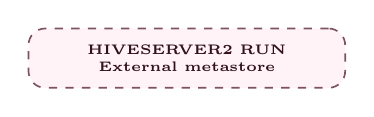
\begin{tikzpicture}
        \node[rounded corners=6pt,draw=MD3Tertiary,line width=0.6pt,dashed,fill=MD3TertiaryContainer!30,align=center,inner sep=6pt,text width=3.6cm,font=\tiny\bfseries,text=MD3OnTertiaryContainer] {HIVESERVER2 RUN\\External metastore};
      \end{tikzpicture}
    \end{column}
    \begin{column}{0.31\textwidth}
      \centering{
\includegraphics[height=0.72cm,keepaspectratio]{pig.png}}\par\vspace{0.12cm}
      \begin{block}{Pig Latin 0.17}
        \tiny
        \texttt{pig/analyze\_events.pig}:\\
        \texttt{LOAD} 5-col TSV $\to$\\
        \texttt{GROUP BY n\_jets} $\to$\\
        \texttt{FOREACH ... COUNT, AVG} $\to$\\
        \texttt{ORDER BY} $\to$ \texttt{STORE}
      \end{block}
      \vspace{0.1cm}
      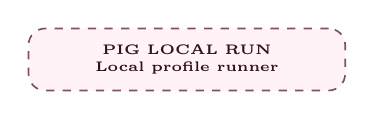
\begin{tikzpicture}
        \node[rounded corners=6pt,draw=MD3Tertiary,line width=0.6pt,dashed,fill=MD3TertiaryContainer!30,align=center,inner sep=6pt,text width=3.6cm,font=\tiny\bfseries,text=MD3OnTertiaryContainer] {PIG LOCAL RUN\\Local profile runner};
      \end{tikzpicture}
    \end{column}
  \end{columns}
  \vspace{0.12cm}
  \tiny\raisebox{-0.05cm}{
\includegraphics[height=0.30cm]{server.png}}\hspace{0.12cm}Spark SQL executes identical queries in core stack; scripts provide standalone portability.
\end{frame}

% ============================================================ S19
\section{Unsupervised Scoring}
\begin{frame}{Streaming MiniBatchKMeans}
  \begin{columns}[T]
    \begin{column}{0.52\textwidth}
      \begin{block}{Model Architecture (10 Features)\hfill\raisebox{-0.12cm}{
\includegraphics[height=0.52cm,keepaspectratio]{scikit.png}}}
        \tiny $\met$, $\HT$, $\STlep$, $N_e$, $N_\mu$, $\njet$, lead $e/\mu/$jet $\pt$, $\max|\eta|$
        \begin{enumerate}
          \item \texttt{StandardScaler.partial\_fit} $\to$ corpus $\mu_j,\sigma_j$
          \item \texttt{MiniBatchKMeans.partial\_fit}, $K{=}8$, rs$=27$
          \item Predict + distance: $s(\mathbf{x}) = \min_k\lVert \mathbf{z}(\mathbf{x})-\boldsymbol{\mu}_k\rVert_2$
        \end{enumerate}
      \end{block}
      \begin{exampleblock}{Full-Corpus Coverage}
        \tiny Rows scaled $=$ fit $=$ scored $=$ 13{,}451{,}915 (100\%); 25.2\,s runtime.
      \end{exampleblock}
    \end{column}
    \begin{column}{0.44\textwidth}
      \begin{block}{Cluster Population ($K{=}8$)}
        \centering
        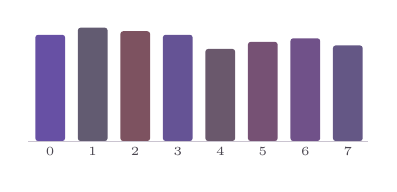
\begin{tikzpicture}[scale=0.9,every node/.style={transform shape}]
          \foreach \x/\h/\l/\c in {0.2/1.5/0/MD3Primary,0.8/1.6/1/MD3Secondary,1.4/1.55/2/MD3Tertiary,2.0/1.5/3/MD3Primary!70!MD3Secondary,2.6/1.3/4/MD3Secondary!70!MD3Tertiary,3.2/1.4/5/MD3Tertiary!70!MD3Primary,3.8/1.45/6/MD3Primary!60!MD3Tertiary,4.4/1.35/7/MD3Secondary!60!MD3Primary}{
            \fill[\c,rounded corners=1pt] (\x,0) rectangle (\x+0.42,\h);
            \node[font=\tiny,MD3OnSurfaceVariant] at (\x+0.21,-0.15) {\l};}
          \draw[MD3OutlineVariant] (0.1,0) -- (4.9,0);
        \end{tikzpicture}
        \tiny Largest: cluster 1 (3.99M) $\cdot$ Smallest: cluster 4 (282k).
      \end{block}
      \begin{exampleblock}{Bounded Memory}
        \tiny \texttt{partial\_fit} streams 25k chunks without loading full corpus into RAM.
      \end{exampleblock}
    \end{column}
  \end{columns}
\end{frame}

% ============================================================ S20
\begin{frame}{Distance Outlier Profiles}
  \begin{columns}[T]
    \begin{column}{0.49\textwidth}
      \begin{figure}
        \centering
        \mdfig{height=0.25\textheight,keepaspectratio}{08_cluster_distance_distribution.png}
        \caption{Distance distribution (full corpus).}
      \end{figure}
    \end{column}
    \begin{column}{0.49\textwidth}
      \begin{figure}
        \centering
        \mdfig{height=0.25\textheight,keepaspectratio}{09_cluster_distance_by_jet_multiplicity.png}
        \caption{Distance conditioned on $\njet$.}
      \end{figure}
    \end{column}
  \end{columns}
  \vspace{0.05cm}
  \begin{columns}[T]
    \begin{column}{0.52\textwidth}
      \mdnum{MD3Primary}{5.2cm}{MD3OnPrimary}{Min 0.224 $\cdot$ Mean 1.648 $\cdot$ $\sigma=0.95$ \\ Max 336.8 $\cdot$ P99 $=$ 4.62}
    \end{column}
    \begin{column}{0.44\textwidth}
      \begin{exampleblock}{Geometric Insight}
        \tiny Median distance grows with $\njet$ ($1.15 \rightarrow 7.12$). Scores isolate complex multi-jet events for targeted expert inspection.
      \end{exampleblock}
    \end{column}
  \end{columns}
\end{frame}

% ============================================================ S21
\section{Synthesis}
\begin{frame}{Evidence Classes \& Quality Guarantees}
  \begin{columns}[T]
    \begin{column}{0.48\textwidth}
      \begin{block}{Four Evidence Classes}
        \tiny
        \begin{itemize}
          \item[\textbf{P}] \textbf{Published Fact}: Zenodo paper / record
          \item[\textbf{C}] \textbf{Calculated Quantity}: Exact verified arithmetic
          \item[\textbf{L}] \textbf{Local Measurement}: JSON manifest values
          \item[\textbf{A}] \textbf{Conditional Artifact}: Generator script outputs
        \end{itemize}
      \end{block}
    \end{column}
    \begin{column}{0.48\textwidth}
      \begin{exampleblock}{Implemented Guarantees}
        \tiny
        \begin{itemize}
          \item Download gates on MD5 and exact byte count
          \item Schema assertion precedes ETL transform
          \item 1:1 row correspondence verified across engines
          \item Unit test assertions on synthetic fixtures
        \end{itemize}
      \end{exampleblock}
    \end{column}
  \end{columns}
\end{frame}

% ============================================================ S22
\begin{frame}{CA3 Course-Outcome Alignment}
  \tiny
  \begin{tabularx}{\textwidth}{p{2.6cm} X p{3.2cm}}
    \toprule
    \rowcolor{MD3SurfaceContainer}
    \textbf{Course Concept} & \textbf{Evidence in Project} & \textbf{Scope Note} \\
    \midrule
    MapReduce & Spark RDD key-value map/reduceByKey, count parity, Hadoop Streaming scripts & Native Hadoop requires external cluster \\
    Hive / SQL & 9 HiveQL queries, partitioned Parquet, grouped stats, Window + ROLLUP & Spark SQL is primary runtime \\
    Pig Latin & GROUP, FOREACH, COUNT, AVG local mode over TSV & Pig 0.17 profile \\
    Spark Columnar & HDF5$\to$Parquet ETL, partitionBy, read-back parity & Single-node Docker \\
    Intelligent Analysis & MiniBatchKMeans novelty score over 10 standardized features & scikit-learn streaming \\
    Visual Analytics & 9 figures: spectra, density, conditionals, correlations, distances & Full-corpus basis \\
    \bottomrule
  \end{tabularx}
\end{frame}

% ============================================================ S23
\begin{frame}{Conclusion \& Caveats}
  \begin{columns}[T]
    \begin{column}{0.54\textwidth}
      \begin{block}{Verified Outcomes}
        \tiny
        \begin{itemize}
          \item 13{,}451{,}915 events audited $\rightarrow$ 0 defects
          \item ETL parity $\rightarrow$ 624.78\,MB Parquet, 539 row groups
          \item 9 SQL groups + RDD aggregation $\sum n_j = N$ \checkmark
          \item $K{=}8$ full-corpus distance scores
          \item 9 figures backed by machine manifests
        \end{itemize}
      \end{block}
      \begin{exampleblock}{Operational Notes}
        \tiny Single-node \texttt{local[6]} executes all queries in 93.8\,s. Upper tail ranks multi-jet topologies for expert inspection.
      \end{exampleblock}
    \end{column}
    \begin{column}{0.42\textwidth}
      \begin{exampleblock}{Key Numbers}
        \centering
        \tiny
        \begin{tabular}{r@{\ }l}
          \toprule
          1{,}022{,}345{,}540 & scalars scanned \\
          82.83\% & structural padding \\
          86.0\% & events with $\njet\le2$ \\
          652.9\,GeV & median $\HT$ @ $\njet{=}10$ \\
          4.62 & P99 centroid distance \\
          93.8\,s & Spark suite runtime \\
          \bottomrule
        \end{tabular}
      \end{exampleblock}
      \vspace{0.1cm}
      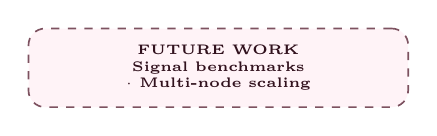
\begin{tikzpicture}
        \node[rounded corners=6pt,draw=MD3Tertiary,line width=0.6pt,dashed,fill=MD3TertiaryContainer!30,align=center,inner sep=6pt,text width=4.4cm,font=\tiny\bfseries,text=MD3OnTertiaryContainer] {FUTURE WORK\\Signal benchmarks $\cdot$ Multi-node scaling};
      \end{tikzpicture}
    \end{column}
  \end{columns}
\end{frame}

% ============================================================ S24
\begin{frame}{References \& Reproducibility}
  \begin{columns}[T]
    \begin{column}{0.55\textwidth}
      \begin{block}{References}
        \tiny
        \begin{itemize}
          \item E.~Govorkova et al., LHC dataset, \emph{Sci. Data} 9:118, 2022.
          \item CERN / Fermilab, Training Dataset, Zenodo 5046428, 2021.
          \item ML for Particle Physics, ADC 2021 Benchmark, 2021.
          \item Apache Software Foundation, Spark 3.5.7 Guides, 2024.
          \item Apache Hadoop $\cdot$ Hive DDL $\cdot$ Pig 0.17 Docs.
          \item Apache Arrow / PyArrow Docs (v18.1.0), 2024.
          \item F.~Pedregosa et al., Scikit-learn, \emph{JMLR} 12:2825, 2011.
        \end{itemize}
      \end{block}
    \end{column}
    \begin{column}{0.41\textwidth}
      \begin{block}{\raisebox{-0.05cm}{
\includegraphics[height=0.32cm]{terminal.png}}\hspace{0.12cm}Reproduce Entire Pipeline}
        \tiny
        \texttt{cp .env.example .env}\\
        \texttt{make build \&\& make test \&\& make all}\\
        \texttt{make check-quality}
      \end{block}
      \begin{exampleblock}{\raisebox{-0.05cm}{
\includegraphics[height=0.32cm]{check.png}}\hspace{0.12cm}Key Verified Results}
        \tiny
        \begin{itemize}
          \item 13.45M events verified with zero scalar defects
          \item Exact row match across Parquet, Spark \& RDD
          \item 93.8\,s single-node Docker reproducibility
          \item Full 100\% unsupervised streaming outlier ranks
        \end{itemize}
      \end{exampleblock}
    \end{column}
  \end{columns}
\end{frame}

\end{document}
